\documentclass{sig-alternate}

% UTF8 support
\usepackage[utf8x]{inputenc}

\usepackage{subfig}
\usepackage{hyperref}
\usepackage{graphicx}
\graphicspath{{figures/}}

\usepackage{booktabs}

\newcommand{\eg}{{\textit{e.g.~}}}
\newcommand{\etal}{{\textit{et al.~}}}
\newcommand{\ie}{{\textit{i.e.~}}}

\usepackage[draft,footnote,nomargin]{fixme}

%
% --- Author Metadata here ---
\conferenceinfo{10th ACM/IEEE International Conference on Human-Robot Interaction}{2015 Portland, USA}
%\CopyrightYear{2007} % Allows default copyright year (20XX) to be over-ridden - IF NEED BE.
%\crdata{0-12345-67-8/90/01}  % Allows default copyright data (0-89791-88-6/97/05) to be over-ridden - IF NEED BE.
% --- End of Author Metadata ---

\title{\LARGE \bf
    Eye-Tracking: a New Look at Human-Robot Interaction Assessment
}

%%% HRI 2015 -> double-blind review process
%
%\numberofauthors{1} 
%\author{
%\alignauthor
%Kshitij Sharma, S\'{e}verin Lemaignan, Pierre Dillenbourg\\
%       \affaddr{Computer-Human Interaction in Learning and Instruction Lab (CHILI)}\\
%       \affaddr{Ecole Polytechnique F\'{e}d\'{e}rale de Lausanne (EPFL)}\\
%       \affaddr{CH-1015 Lausanne}\\
%       \affaddr{Switzerland}\\
%       \email{firstname.lastname@epfl.ch}
%}
%
%\additionalauthors{Additional authors: 
%Francesco Mondada, LSRO, EPFL, francesco.mondada@epfl.ch 
%}
%

\begin{document}
\maketitle
\begin{abstract}


Eye-tracking has been previously shown to be an effective proxy to understand
complex socio-cognitive interactions. Yet its application to human-robot
interactions (HRI) remains limited. This article presents the state of the
art in eye-tracking methods for interaction assessment, and explores how those
are applicable to HRI.

Techniques based on mobile eye-tracking as well as the main analysis approaches
for eye-tracking data are first exhaustively presented, with an emphasis on
those we believe relevant to robotics. We then report on a study involving the
educational robot Thymio II~\cite{riedo2012two} with 52 participants: the
students have to explain a pre-programmed behaviour of the robot with or without
the help of visual cues. The study setup and analysis illustrate how to apply
eye-tracking techniques to actual human-robot interaction situations.

\end{abstract}
%%%%%%%%%%%%%%%%%%%%%%%%%%%%%%%%%%%%%%%%%%%%%%%%%%%%%%%%%%%%%%%%%%%%%%%%%%%%%%%%%%%%
%%%%%%%%%%%%%%%%%%%%%%%%%%%%%%%%%%%%%%%%%%%%%%%%%%%%%%%%%%%%%%%%%%%%%%%%%%%%%%%%%%%%
\section{Introduction}

Eye tracking provides unprecedented access to the users' attention and
engagement during interactive scenarios. Previous research
\cite{hasse2012measure,tien2010measuring,jermann2010using,sharma2012gaze} has
shown that gaze data can be used as a proxy to understand the underlying
socio-cognitive aspects in not only human-computer interaction but in
human-human interaction as well. In the present decade, off the shelf
eye-trackers have become readily available to the researchers to assess the
users' attention and engagement.



\paragraph{Biometric Measurements of Interaction}

Evaluation of HRI is mostly done through qualitative questionnaires and
qualitative data (interaction videos, interviews for example). The physiological
measurements such as eye tracking being precise, pertinent and portable at the
same time provides an added value to the researcher.  Eye-tracking data is of
high temporal precision as compared to some of the physiological data sources
such as fMRI or other biometric devices used to measure the palpitation and the
body temperature. The eye tracking devices are portable enough as opposed to the
bulky apparatus used in fMRI~\cite{rosenthal2013neural}. Eye tracking data
provides more direct access to the users' attention than other portable and
physiological data sources such as EEG and wristbands measuring skin conductance
and pulse rate; this makes eye-tracking data a pertinent source to measure
attention.

The prime advantage of using mobile eye-tracking is that the users' interaction
with the robot can still be ecologically valid. On the other hand, using fMRI
for evaluating HRI reduces the interaction to a video of the robot
only~\cite{rosenthal2013neural}.

Another advantage of using mobile eye-tracking to assess HRI situations, is that
the data provides direct and noise free access to the users' attention. While in
other physiological measures for attention, such as EEG, the data has a lot of
noise and the relation to the attention is very task-specific.

In a nutshell, the use of gaze data as an assessment of the human-robot
interaction in an educational setting provides future research prospects. The
data acquisition is a better trade-off between the ecological validity of the
experiment (as there cannot be an interaction with the robot fMRI data
acquisition) and the precision of the data stream (wristbands for measuring the
palpitation and the temperature).

\paragraph{Article overview}

The article is structured as follow: section~\ref{et_assessing} presents the
main lines of research in eye-tracking-based assessment of cognitive
tasks and interaction. It evidences the breadth of the field, both on individual
and social tasks. Section~\ref{et_robotics} contrasts this literature with the
current state-of-the-art of eye-tracking in HRI. We distinguish here two main
applications: eye-tracking as an \emph{interaction modality} and eye-tracking as
an \emph{interaction assessment} tool. It appears that the literature in both
these fields is scarce.

Section~\ref{method} presents in a brief yet exhaustive way eye-tracking as an
investigation method: we introduce the main eye-tracking techniques (including
mobile eye-tracking and dual eye-tracking) and discuss their respective domains
of application. We then present five important techniques for eye-tracking data
analysis and emphasise the analysis techniques that are the most relevant to the
study of social interaction.

Next, section~\ref{application} presents a case study with 52 subjects
interacting with a robot. The study acts both as a demonstration of the
integration of eye-tracking in HRI studies, and as an example of a possible
eye-tracking setup. Then, section~\ref{interpretation} goes over the analysis of
the study data and its interpretation, and illustrates this process.

We conclude the article with a summary of the strengths of eye-tracking to
analyse the complex socio-cognitive situations that characterise human-robot
interaction, as well as a few notes on the limitations of this method.


%%%%%%%%%%%%%%%%%%%%%%%%%%%%%%%%%%%%%%%%%%%%%%%%%%%%%%%%%%%%%%%%%%%%%%%%%%%%%%%%%%%%
%%%%%%%%%%%%%%%%%%%%%%%%%%%%%%%%%%%%%%%%%%%%%%%%%%%%%%%%%%%%%%%%%%%%%%%%%%%%%%%%%%%%
\section{Eye Tracking as a Tool for Assessing Social Interaction}
\label{et_assessing}

\subsection{Gaze patterns and Expertise/Task based performance}

Several scholars related gaze patterns with level of expertise.
\cite{hasse2012measure} in an air traffic-monitoring task found out that the
experts looked less at the scenario-specific information than novices.
\cite{eivazi2012gaze, law2004eye, tien2010measuring} studied the effect of
expertise on the gaze patterns in different surgical tasks and concluded that
experts look less at the instruments than the novices, instead they focus more
on the task specific areas. \cite{reingold2001visual} showed that expert chess
players pay more attention to the relative positions of the pieces, rather than
the individual pieces, than novice chess players. \cite{blignaut2008visual} also
studied the difference between experts and novice chess players in a checkmate
avoidance task and concluded that the experts have more gaze falling on the
important squares than the novices. In a program-debugging task,
\cite{sharif2012eye} showed that the expert programmers scan through all the
lines in the program faster than the novices. In a Tetris game,
\cite{jermann2010using} showed that experts pay more attention to the stack of
Tetronimoes while novices allocate more attention to the new pieces falling from
the top.

\subsection{Gaze patterns and Collaborative performance}

Previous work also show a clear relation between gaze patterns and task-based
performance in collaborative settings. As a measure of joint attention in
collaborative settings  \cite{richardson2007art} proposed gaze recurrence
between the collaborators and showed it to be correlated with the collaboration
quality of the pair. In a pair-programming task, \cite{jermann2012effects}
showed that the good performing pairs have more synchronised gaze on different
parts of a program than the bad performing pairs. In a similar task,
\cite{sharma2012gaze} showed that the good performing pairs pay more attention
to the data-flow of the program than the poor performing pairs. Moreover,
\cite{sharma2013understanding} showed that while describing the functionality of
a program the well performing teams had more gaze on the variable modification
parts in the program while poor performing teams have equal distribution of gaze
on different parts of the program during similar phase of the task.  Thus we see
that previous research provides insights about the relationship between the gaze
patterns and the behavioural and task-based performance indicators in diverse
scenarios.

%%%%%%%%%%%%%%%%%%%%%%%%%%%%%%%%%%%%%%%%%%%%%%%%%%%%%%%%%%%%%%%%%%%%%%%%%%%%%%%%%%%%
%%%%%%%%%%%%%%%%%%%%%%%%%%%%%%%%%%%%%%%%%%%%%%%%%%%%%%%%%%%%%%%%%%%%%%%%%%%%%%%%%%%%


\section{State of Eye Tracking in Human-Robot Interaction}
\label{et_robotics}

The usage of eye-tracking methods in HRI is very sparse. It must be noted that
to our best knowledge only very few attempts to use eye-tracking as an
interaction modality or as an interaction assessment technique in HRI.

\subsection{Eye Tracking as an Interaction Modality}

To guide the motion of a robot \cite{bhuiyan2004tracking} used real time  gaze
data of a human user. The users were able to provide the visual and geometrical
motion information to the robot by moving their eyes in different parts of the
human-robot interface.

\subsection{Eye Tracking as a tool to Assess Interaction Algorithms}

To evaluate the effectiveness of the motion planning algorithm for a robot
\cite{dehais2011physiological} used eye-tracking techniques. In an object
hand-over task between a robot and a human, the authors compared various motion
planning algorithms based on the gaze of the human.

\subsection{Eye Tracking as a tool to Assess Joint Attention}

In an eye-tracking study, in the context of human robot interaction,
\cite{staudte2009visual} found that when the robot provides a matching visual
and verbal reference to an object the participants were more likely to look at
the correct objects. This result was consistent irrespectively of the ambiguity
of the situation. The video based interaction modality was used by the authors.
This constraints the  interaction of the human-robot dyad to just a video.
However, the stimulus (video) for eye-tracking provides strong contrast and a
good control for experimental conditions.


%%%%%%%%%%%%%%%%%%%%%%%%%%%%%%%%%%%%%%%%%%%%%%%%%%%%%%%%%%%%%%%%%%%%%%%%%%%%%%%%%%%%
%%%%%%%%%%%%%%%%%%%%%%%%%%%%%%%%%%%%%%%%%%%%%%%%%%%%%%%%%%%%%%%%%%%%%%%%%%%%%%%%%%%%

\section{Method description}
\label{method}

\subsection{Eye-tracking}
First, we introduce the basic eye-tracking setups, technical steps in mobile eye-tracking and different use cases of mobile eye-tracking.

\subsubsection{Apparatus}

Most eye trackers work by projecting infrared light on the pupil and measuring the reflection with one or more cameras. . Following are the typical setups for the eye-trackers used in research:


\begin{enumerate}
\item Stationary: The stationary eye-trackers are widely used for the controlled laboratory experiments. These eye-trackers have a separate eye-tracking device (camera, infrared source and microprocessor) and a monitor or a monitor embedded with different parts  of the eye-tracking devices. The data rate is usually higher than the mobile eye-trackers (ranging between 60 Hz to 2000 Hz). The accuracy of current devices is about 0.5 degrees, which correspond to 0.35 mm for a user whose head is placed at 40 cm from the screen.  The setup needs the heads of the participants to be fixed using a opthalmologic head rest for better data quality. 

\item Mobile: Mobile eye-trackers are useful to conduct more ecologically valid and naturalistic experiments. These eye-trackers have a scene camera in the front to record the visual field of the participants. Present mobile eye-trackers have a data rate of 30 Hz and a spatial accuracy equal to the stationary eye-trackers.

\item Dual eye-tracking: Dual eye-tracking requires synchronisation of two eye-trackers, so that the researchers can record the gaze data for a pair of collaborators without any lag (as the clocks of two systems can not be perfectly synchronised). \cite{nussli2011dual} explored and compared different ways to synchronise two eye-trackers.

\end {enumerate}


\subsubsection{Mobile Eye-tracking setup}

\begin{enumerate}
\item Calibration
\item Recording Scene 
\item Recording Gaze

\end {enumerate}

\subsubsection{Use cases for mobile eye-tracking} 

\begin{enumerate}
\item Stationary target, stationary observer
\item Moving target, stationary observer
\item Stationary target, moving observer
\item Moving target, moving observer
\end{enumerate}


\subsection{Data and Analysis}

\begin{enumerate}
\item Fixations: The most common form of eye-tracking data aggregation are the fixations. Fixations depict the periods in the user's observation when the user attends a relatively small part of the visual stimulus for a relatively longer period of time. The various fixation detection algorithms are summarised in~\cite{duchowski2007eye}. 

\item Saccades and transitions: Two fixations are connected by a saccade. Saccades are the sudden variations in the eye-movements. While analysing saccades, there are two 
\item Smooth Pursuit
\item Areas of Interest
\item Heat-maps

\end {enumerate}


\subsection{Analysing social behaviour}

\begin{enumerate}
\item Joint attention
\item interaction episodes
\end{enumerate}


%%%%%%%%%%%%%%%%%%%%%%%%%%%%%%%%%%%%%%%%%%%%%%%%%%%%%%%%%%%%%%%%%%%%%%%%%%%%%%%%%%%%
%%%%%%%%%%%%%%%%%%%%%%%%%%%%%%%%%%%%%%%%%%%%%%%%%%%%%%%%%%%%%%%%%%%%%%%%%%%%%%%%%%%%

\section{Method Application Example}
\label{application}

In this section, we present a mobile eye-tracking study with an educational
robot Thymio II. The study exemplifies one of the use cases of the mobile
eye-tracking. One part of the target (the robot) was moving, whereas the rest of
the maze (or playground, figure~\ref{playground}, as we refer to it in the rest
of this paper) was stationary. The participants were allowed to move but most of
them remained seated for the duration of the experiment. For the purpose of the
eye-tracking data analysis, we used the proportions of fixations on different
area of interest on the playground.

We propose to use the mobile eye trackers to be able to have our participants
freely move on the experiment site. Using mobile eye tracker poses a technical
challenge to automatically locate where the participants are looking. This is
not a trivial task as the visual stimulus for participants is changing with
every bit of motion of their head. This is the reason we used fiducial-markers
on the maze we used in the experiment so that we can reconstruct the whole maze
even if only a part of it is the visual field of the participant.

\subsection{Setup and Conditions}

Thymio II is a small robot designed for education for 6 to 16 year old
children~\cite{magnenat2012programming, riedo2012two}. Users can interact with
it via buttons and distance sensors. The robot can display its states via many
LEDs and its motion. We programmed it to show the value of the front IR-sensor
on its top. The display consists of 8 LEDs (Figure~\ref{thymio}).

In the experiment, there were 3 sensor data visualisation conditions.  For the
{\sf TRUE} visualisation condition, the number of illuminated LEDs, on the top of the
robot, is proportional to the intensity measured by the IR-sensor. When the
intensity of the reflected IR crosses a predefined threshold, the robot does a
90° turn to its right. For the two other conditions, the behaviour is the same,
simply the display changes. In the {\sf RANDOM} condition, the display shows as if the
robot was detecting the obstacle at random moments, while in the {\sf NONE}
visualization condition nothing is shown on top of the robot. The robot has a
fitting for a pencil that we used for the drawing of its trajectory.

\begin{figure}
    \centering
    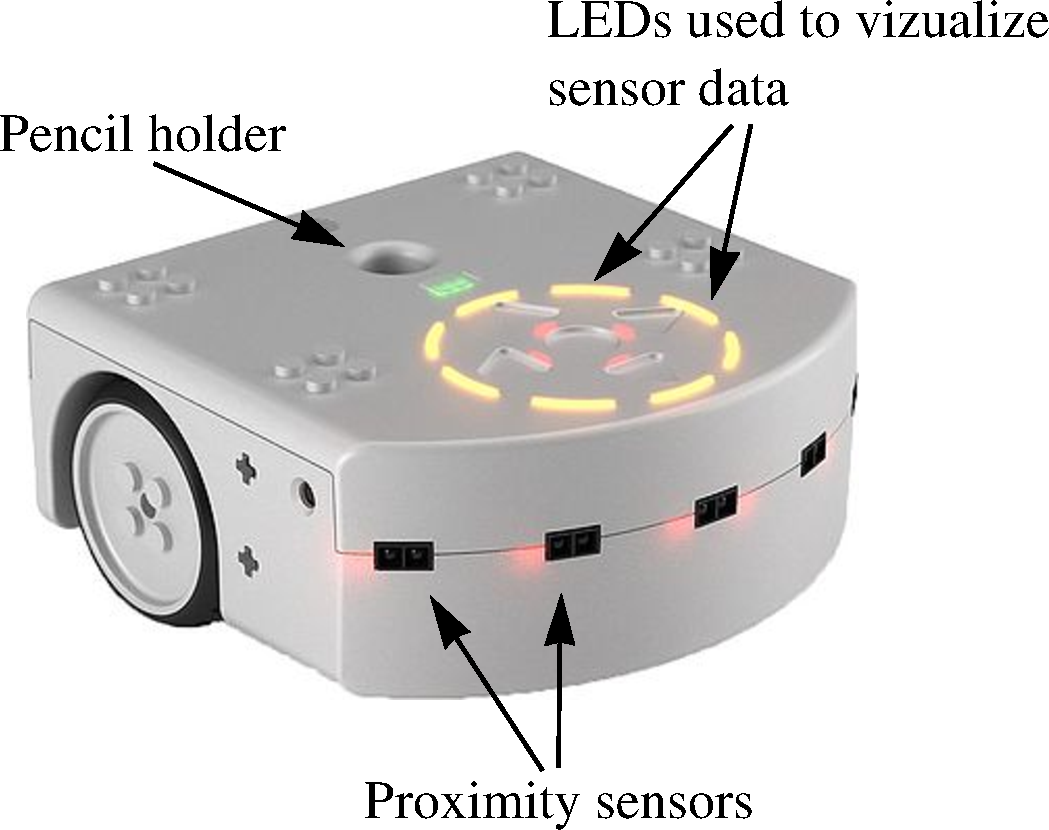
\includegraphics[width=0.9\linewidth]{thymio}
    \caption{\small \textbf{Thymio II}: the proximity sensors were used to
    detect the obstacle based on the reflectance of the material. The sensor
    data was shown as a proportion of the circle lit using the LEDs on top of the
    robot.}

    \label{thymio}
\end{figure}

The playground (Figure~\ref{playground}) is designed in order to allow the
participants to get a reference of the previous behaviour of the robot, as well
as to allow us to localise the position of the robot, the position of the
obstacles and the position of the gaze on the video recorded from the
eye-tracker. The localisation is made possible by the use of unique fiducial
markers on the playground. On the right hand side, the observation phase takes
place and there will be the reference for the black and white obstacles. On the
left hand side, the interaction takes place.

\begin{figure}
    \centering
    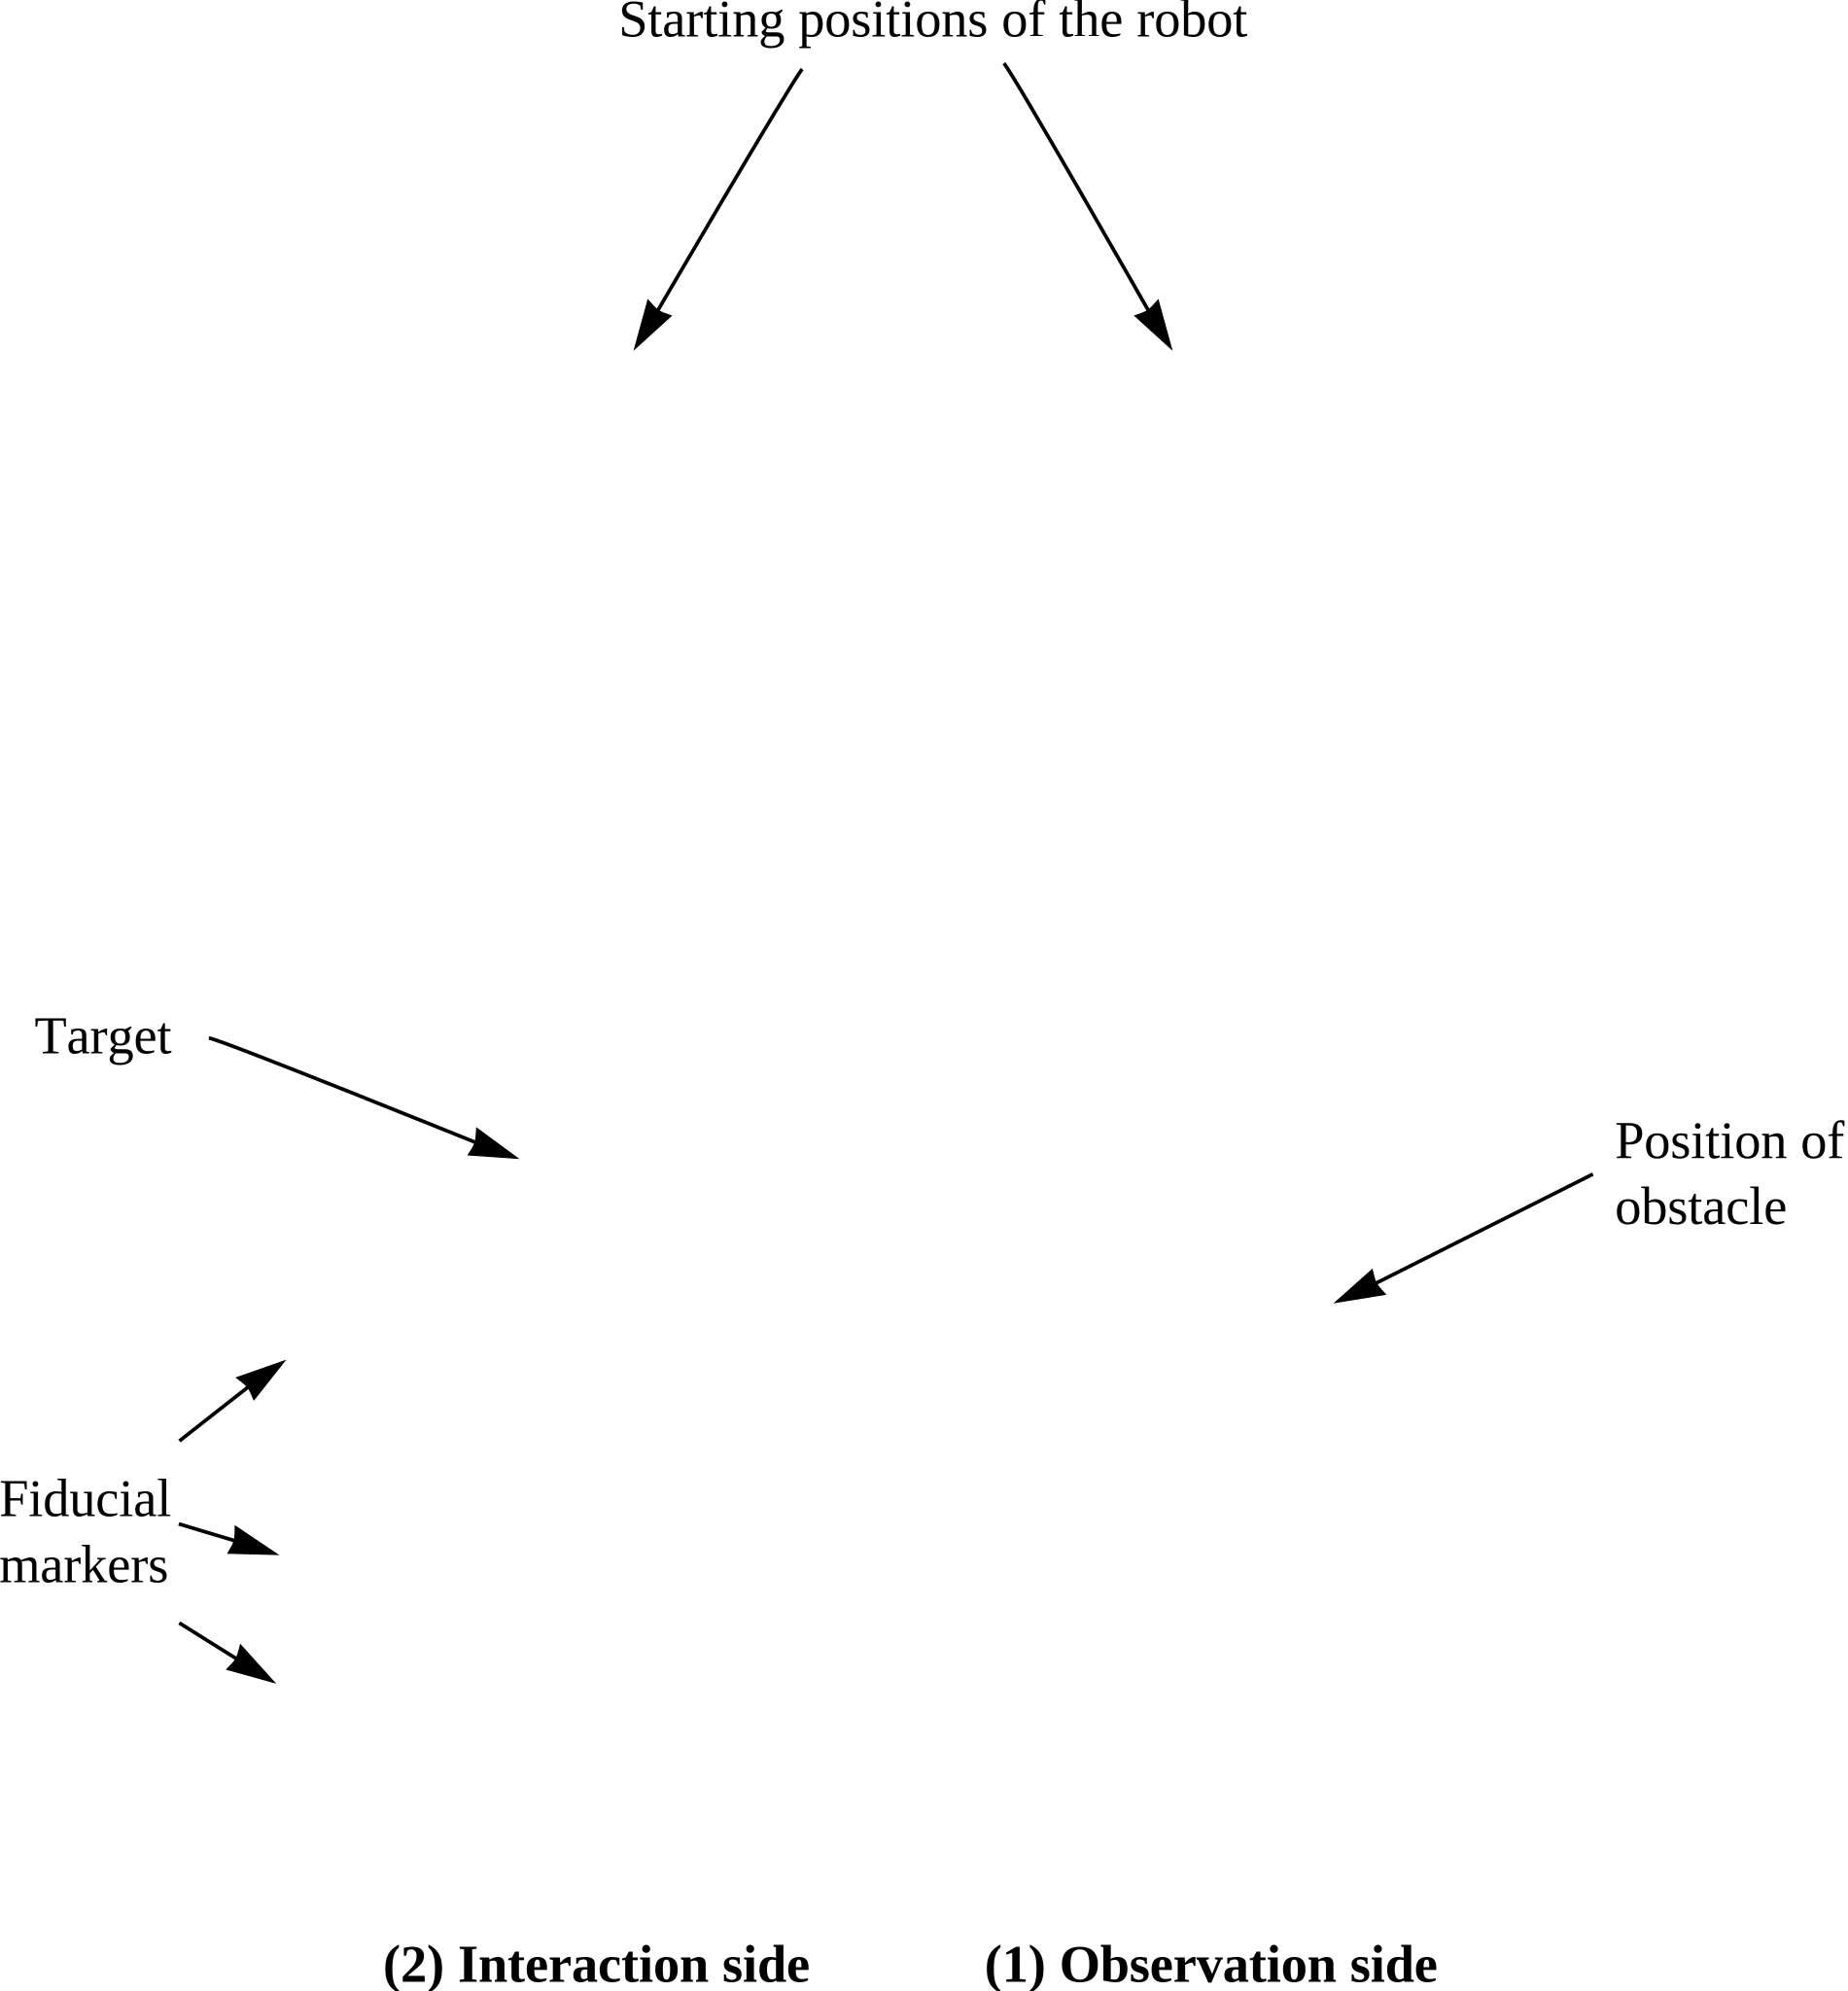
\includegraphics[width=0.9\linewidth]{maze}
    \caption{\small Basic playground for the experiment. The fiducial markers
    are used for automatic localisation of the gaze pointers on the observation
    video.}

    \label{playground}
\end{figure}

One important fact to be considered is that the localisation of the
robot, the obstacle or the gaze pointer on the observation field for the
participant is not a trivial task. The fact that the participants are
free to move, poses a challenge to the eye-tracking analysis. The
movement of the participant causes change in the observation field of
the participant almost every frame of the eye-tracking video. To cope up
with the changing observation field we decided to put an array of
fiducial markers on the playground. Using the fiducial markers enabled
us to recreate the whole playground for every frame in the video
recorded from the eye-tracker's camera (Figure~\ref{expe}).

\subsection{Procedure}

Upon their arrival at the experiment site, the participants signed a consent
form and answered a small questionnaire about demographics and participant's
experience with educational robots (this we later consider as expertise). The
participants were placed in front of the playground (Figure~\ref{expe}) and were
equipped with the SMI eye-tracking glasses. The eye-tracker records the gaze
data at 30Hz with an accuracy of 0.5 degrees at 40 centimetres distance; and the
scene camera of the eye-tracking glasses records the video in HD.  The actual
experiment consisted in two phases: observation phase and interaction phase.

\paragraph{Observation phase} The participant observes the Thymio II robot
approaching obstacles. The robot turns as soon as it detects the
obstacle. The participant watches the robot's behaviour for a black and a
white obstacle for 5 trials each. For the white, the robot turns
earlier; for the black obstacle the robot turns later. In the final
trial the robot is equipped with a pen to draw its trajectory for both
obstacles with different colours. After drawing, the participant is asked
the question: ``How does the robot work?''

\paragraph{Interaction phase} In the second phase, the participant is asked
to guide the robot to a goal, using a grey obstacle. The participant can put the
obstacle wherever he likes on the left hand side (Figure~\ref{playground}) of
the playground before the robot starts. We designed the grey obstacle to reflect
more infrared light (IR) than the black or the white obstacles therefore the
robot turns even earlier. This leads to a surprising effect. The participant has
only the robot's trajectories as a source of information. Each participant is
given 5 trials to put the obstacle in order to guide the robot to the goal. The
participant then has to answer the same question as in the observation phase,
response to which is considered as a final answer.

\begin{figure}
    \centering
    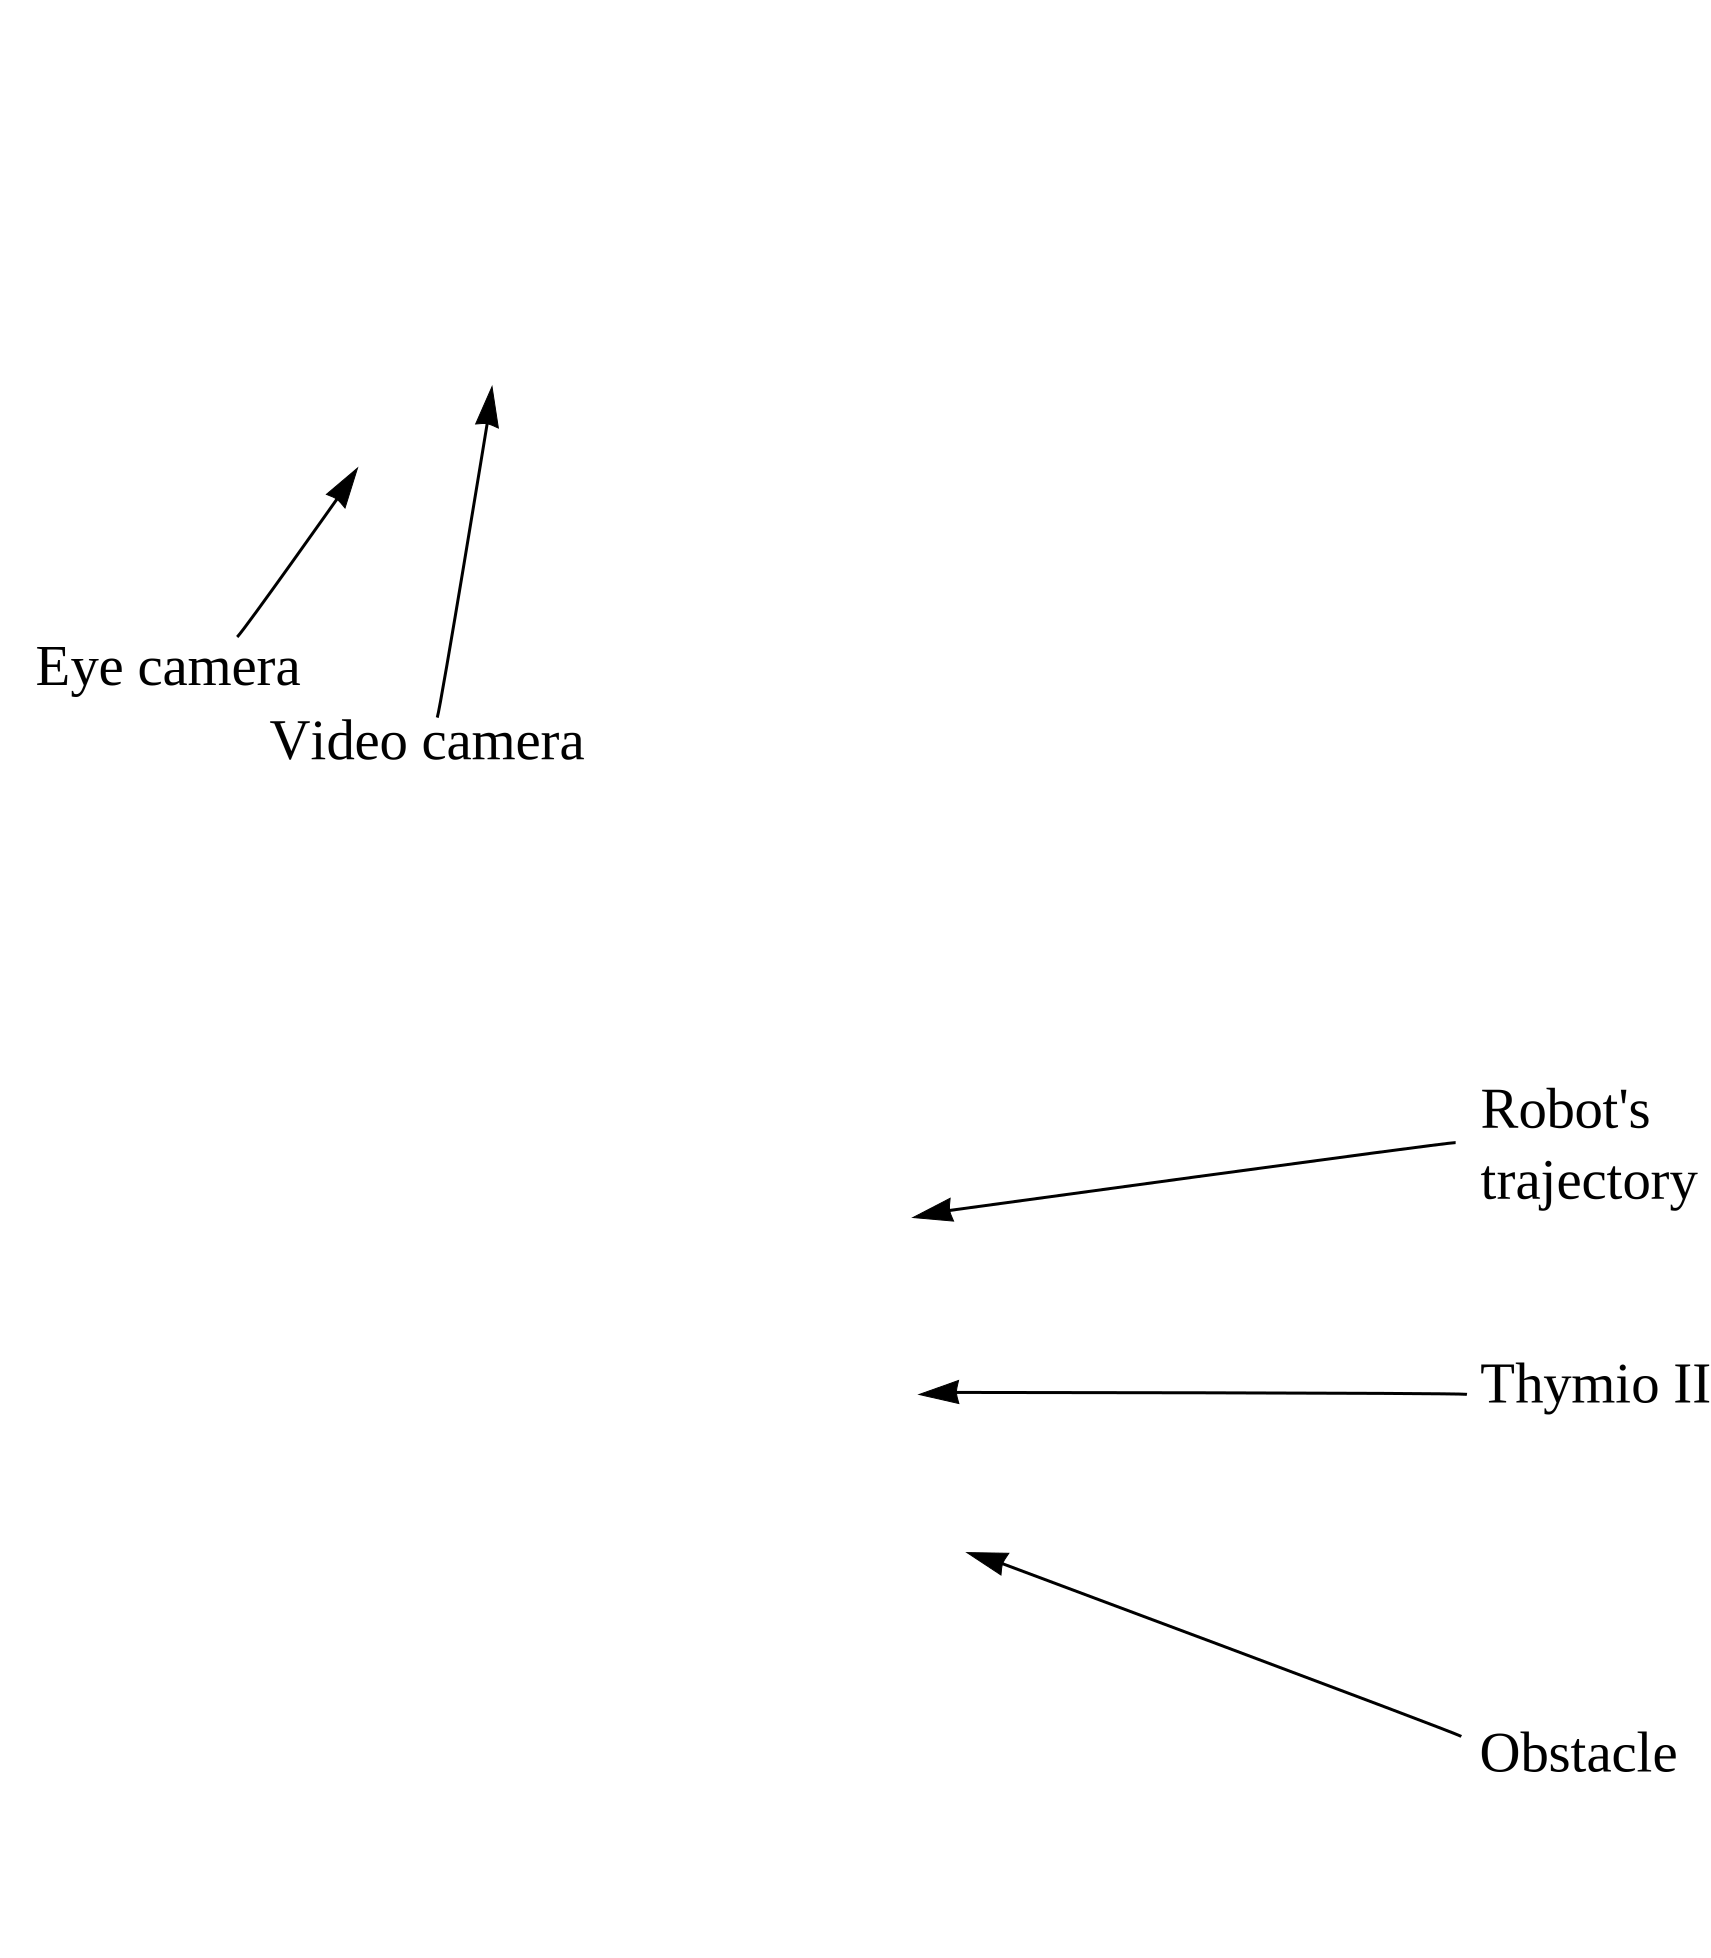
\includegraphics[width=0.9\linewidth]{setup}
    \caption{\small Experimental setup for observation phase. The observation
    video is recorded from the video camera in the front of the eye tracker (in
    the lop-left corner).}

    \label{expe}
\end{figure}

\subsection{Participants}

We recruited 52 participants for the experiment. All of them were
students from École Polytechnique Fédérale de Lausanne, Switzerland.
Most of them were in their first year undergraduate program (with two
exceptions). ~The age distribution was narrow, with a mean of 19.7 and a
standard deviation of 1.97. There were 13 female and 39 male
participants. In the three experimental conditions, {\sf NONE}, {\sf RANDOM} and
{\sf TRUE}, there were 18, 17 and 17 participants respectively.

\subsection{Eye-tracking measures}

Average fixation duration on the robot: We measured the amount of time a
participant looks at the robot and averaged this duration for the number
of fixations on the robot for the particular participant.

Average fixation on the reference side: The main area (right hand side
of figure 2) in the observation phase is treated as the reference side
in the interaction phase. The rationale behind keeping the lines drawn
by the robot in the observation phase is for the participants to be able
to refer to the prior behaviour of the robot in the interaction phase. We
measured the amount of time a participant looks at the reference side
and averaged this duration for the number of fixations on the reference
side for the particular participant.

\subsection{Performance measures}


We measured the distances from the target were measured for all 5 trials. As
a matter of fact, as soon as the principle of the robot was deemed to be
understood by the participants, almost all the participants behaved the
same way. On the first try almost every participant failed and the robot
turned instantly. So the most significant distance measure was the
improvement between the first and second trial. It is referred to as
improvement in the following sections.



%%%%%%%%%%%%%%%%%%%%%%%%%%%%%%%%%%%%%%%%%%%%%%%%%%%%%%%%%%%%%%%%%%%%%%%%%%%%%%%%%%%%
%%%%%%%%%%%%%%%%%%%%%%%%%%%%%%%%%%%%%%%%%%%%%%%%%%%%%%%%%%%%%%%%%%%%%%%%%%%%%%%%%%%%

\section{Interpreting the Results}
\label{interpretation}

\subsection{Results}

We found no bias for age, gender, expertise, student status or condition
in respect to the correctness, abstraction and type of mistake made for
the final answer. Surprisingly there is no correlation between the
visualisation condition and the correctness or abstraction of the
answers given. We could not find any anticipation patterns in the
eye-tracking data. We found some other relation between the different
measures. We present the results in following subsections.

\subsubsection{Average fixation duration on the robot during observation phase
vs.~condition}

The average fixation duration on the robot during observation phase
(Figure~\ref{res1}) is significantly more in {\sf TRUE} and {\sf RANDOM} condition than in
the {\sf NONE} condition ($F[2,49]=3.68$, p = .03). This depicts that the
sensor data visualisation has an effect on the users' attention.

\begin{figure}[h!]
    \centering
    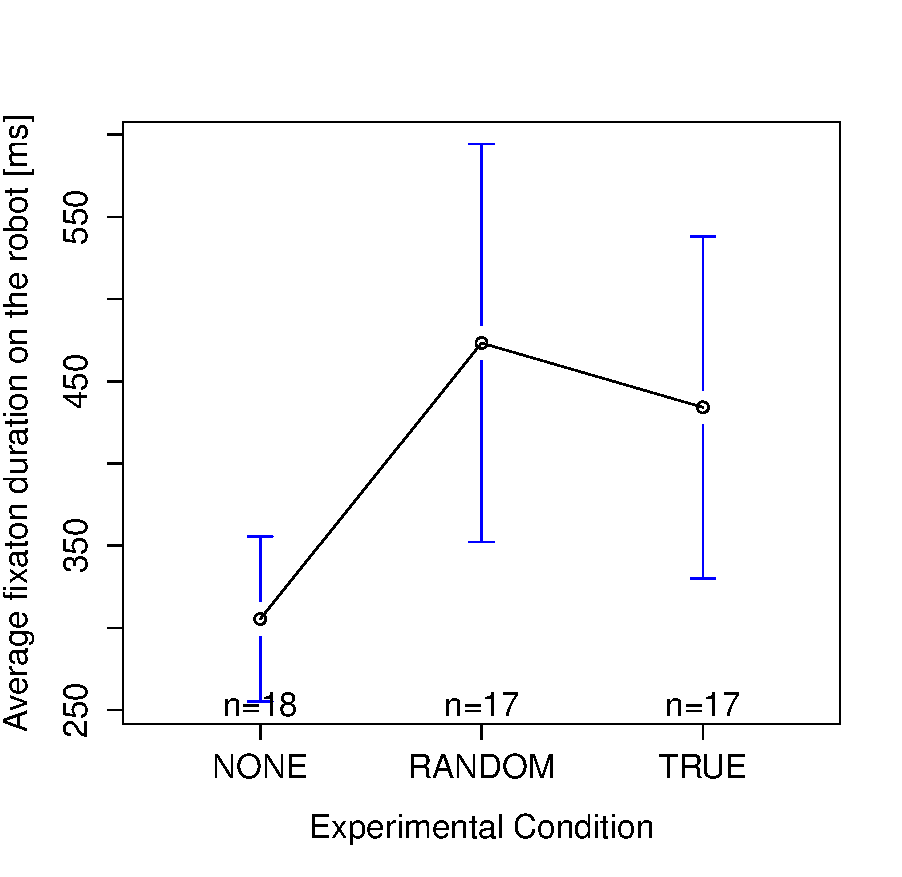
\includegraphics[width=0.8\linewidth]{meanPlotFixRobo}
    \caption{Average fixation duration on the robot ~during the observation phase
    vs.~Condition}
    \label{res1}
\end{figure}

\subsubsection{First improvement vs.~condition}

The first improvement is significantly more in {\sf NONE} and {\sf RANDOM}
conditions (Figure~\ref{res2}) than in the {\sf TRUE} condition ($F[2,49]=3.75$, p =
0.03).

\begin{figure}[h!]
    \centering
    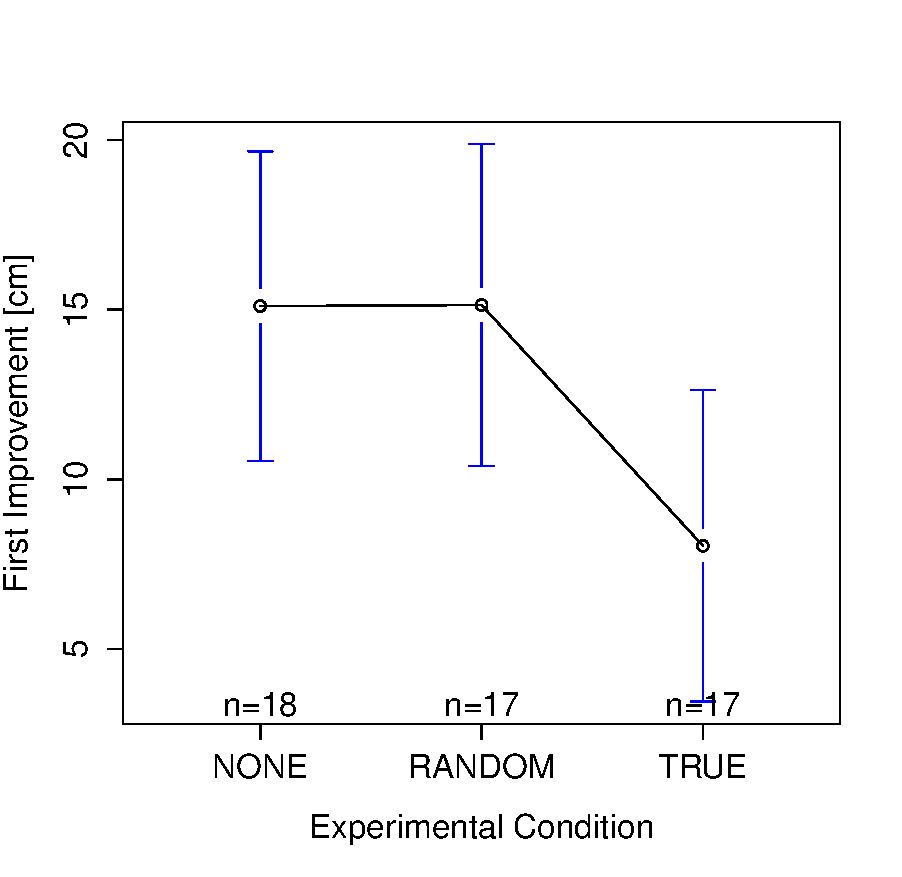
\includegraphics[width=0.8\linewidth]{meanPlotFirstImprove}
    \caption{First improvement vs.~experimental condition}
    \label{res2}
\end{figure}

\subsubsection{Average fixation duration on the reference side during interaction
phase vs.~condition}

The average fixation time on the reference side of the playground
(Figure~\ref{res3}) during the interaction phase is significantly more in {\sf NONE}
and {\sf RANDOM} condition than it is in the {\sf TRUE} condition ($F[2,49]=4.19$,
p = .02).

\begin{figure}[h!]
    \centering
    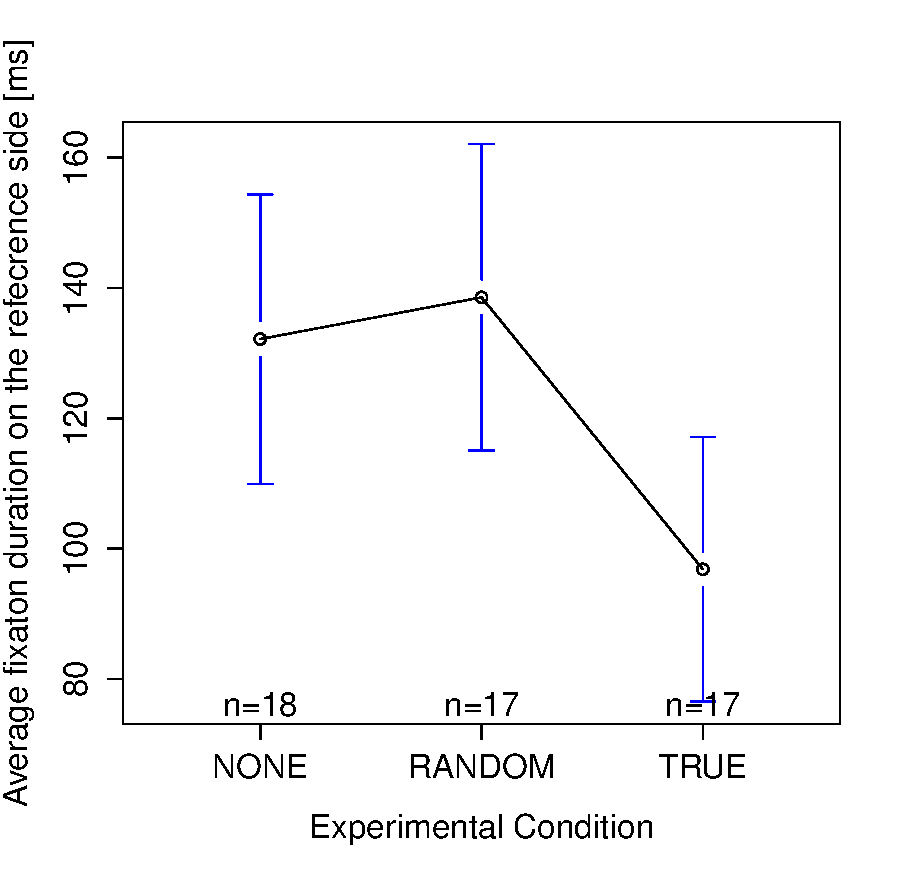
\includegraphics[width=0.8\linewidth]{meanPlotFixReference}
    \caption{Average fixation duration on the reference side during the
    interaction phase vs.~Condition}
    \label{res3}
\end{figure}

\subsubsection{First improvement vs number of fixations on reference side}

There is a significant negative correlation between the number of
fixations on the reference side (Figure~\ref{res4}) during the interaction phase
and the first Improvement ($t(50)=-2.13$, Pearson's correlation = -0.29, p=.03).

\begin{figure}[h!]
    \centering
    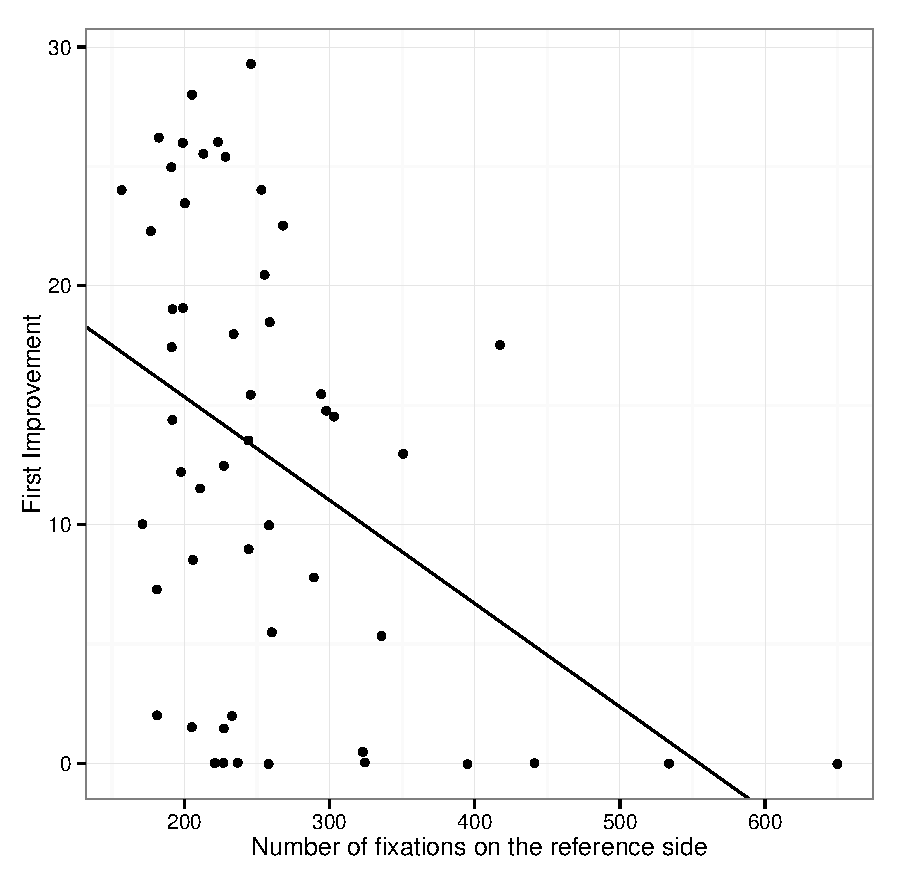
\includegraphics[width=0.8\linewidth]{corPlotFirstImprove}
    \caption{First improvement in centimeters ($y$-axis) vs.~number of fixations
    on reference side ($x$-axis) during the interaction phase.}
    \label{res4}
\end{figure}

%%%%%%%%%%%%%%%%%%%%%%%%%%%%%%%%%%%%%%%%%%%%%%%%%%%%%%%%%%%%%%%%%%%%%%%%%%%%%%%%%%%%
%%%%%%%%%%%%%%%%%%%%%%%%%%%%%%%%%%%%%%%%%%%%%%%%%%%%%%%%%%%%%%%%%%%%%%%%%%%%%%%%%%%%

\subsection{Interpretation}

We present an exemplar eye-tracking study in the context of human-robot
interaction within an educational setting. In this section we give an example of
"how to interpret the eye-tracking results". The fact that participants have
higher average fixation duration on the robot during the observation phase in
the {\sf NONE} condition than the other two conditions (Figure 4) is not
surprising as displaying visual information on the robot induces a saliency
effect on the attention and the gaze is attracted towards the salient feature in
the field of view. 

The fact that the participants in the {\sf RANDOM} or {\sf NONE} visualisation
condition improved more than those with {\sf TRUE} condition is surprising
(Figure 5). There are two plausible explanations. The first is that participants
who see the robot in the {\sf TRUE} condition have a stronger belief that the
robot always behaves the same. They see the LEDs of the robot turning on and
therefore the robot still works. The ones with {\sf NONE} visualisation do not
have an indication whether the robot works the same way as in the observation
phase, and start experimenting earlier. The second explanation is that the
participants in {\sf TRUE} condition just put the obstacles out of detection
range, because they could see different display information and concluded
therefore it may behave differently.

The fact that the participants in the {\sf RANDOM} or {\sf NONE} visualisation
condition improved more than those with {\sf TRUE} condition is surprising
(Figure 5). There are two plausible explanations. The first is that
participants who see the robot in the {\sf TRUE} condition have a stronger
belief that the robot always behaves the same. They see the LEDs of the
robot turning on and therefore the robot still works. The ones with {\sf NONE}
visualisation do not have an indication whether the robot works the same
way as in the observation phase, and start experimenting earlier. The
second is that the participants in {\sf TRUE} condition just put the obstacles
out of detection range, because they could see different display
information and concluded therefore it may behave differently.

The fact that participants have lower average fixation duration on the
reference side in the interaction phase in the {\sf TRUE} condition than the
other two conditions actually supports the explanation that participants
with {\sf TRUE} condition had a higher initial belief in their cognitive model
of how does the robot work (Figure 6). They did not need to look onto
the reference given in observation phase. This also verifies our working
hypothesis that a carefully designed mapping between the robot's
behaviour and its visual actuators can help in maximising the learning
effect during the interaction.

%%%%%%%%%%%%%%%%%%%%%%%%%%%%%%%%%%%%%%%%%%%%%%%%%%%%%%%%%%%%%%%%%%%%%%%%%%%%%%%%%%%%
%%%%%%%%%%%%%%%%%%%%%%%%%%%%%%%%%%%%%%%%%%%%%%%%%%%%%%%%%%%%%%%%%%%%%%%%%%%%%%%%%%%%

\section{Conclusion}
\label{conclusion}

The task that we have presented was initially motivated by those two questions:

\begin{enumerate}
    \item Can we characterise the participants' behaviours that
        lead to good performance during the interaction? In particular, do
        we observe any anticipation patterns for the good performers?

    \item How does visual cue affects the performance of the participants?

\end{enumerate}

The task was performance-oriented and yet we were interested in accessing and
understanding the cognitive mechanisms at stake during the interaction: where do
participants look when they want to understand a robot behaviour? Does
\emph{anticipation} reflect understanding? How the robot's design impact the
interaction?

We believe that mobile eye-tracking, as a relatively non-invasive yet accurate
(both spatially and temporally) biometric measurement, is a key tool to
investigate this kind of questions in ecologically valid environments.

In that regard, we identify three main strengths of eye-tracking. First,
eye-tracking introduce less experimental bias: mobile eye-tracker are
non-invasive and lightweight. Combined with mobile recording units, they do not
put any constraints on participant movements, contrary to traditional techniques
like video recording. Also, contrary to questionnaires or interview-based
protocol where the experimenter active role may influence the assessment,
eye-tracker are easy to ``forget about'' for the participants.

Second, eye-tracking provides a direct, un-mediated access to the subject's
attentional focus~\cite{sharma2014withmeness} (both spatially -- where does the
subject look at -- and temporally -- where does the subject's attention stays).
Importantly, this information leads to a fine-grained measure of
\emph{engagement}.  Also, the good temporal resolution of eye-trackers allows
for the accurate study of the \emph{dynamics} of attention: what are the
attentional patterns of the subject during the interaction.

Third, it has been showed in literature that eye-tracking can provide an
effective measure of higher socio-cognitive behaviours: it can be used as a
predictor for successful joint task achievement~\cite{sharma2013understanding},
or as a measure of \emph{interaction quality}~\cite{jermann2012effects} through
measurement of joint attention.

One need however to be aware of its limitations: eye-tracking does not give a direct
access to underlying mental representations, and a gaze pattern does not
automatically tell us what the subject think of (EEG or fMRI may be slightly
closer to that target, but they come with their own range of limitations).

Besides, mobile eye-tracking come with an additional cost. As
we mentioned earlier, the automatic localisation of the gaze pointer on
the visual stimulus is not a trivial task. In our study, we relied on a 
number of fiducial markers to the playground, but they were reported as
distractive by the participants. More complex computer vision tools (object
tracking) can alleviate the need for such markers, but it certainly requires
significant pre-processing prior to data analysis.

Still, we believe that eye-tracking, as a method for the assessment and
understanding of the complex cognitive mechanisms that underlie human-robot
interaction, is a promising tool, currently under-used in robotics.



%%%%%%%%%%%%%%%%%%%%%%%%%%%%%%%%%%%%%%%%%%%%%%%%%%%%%%%%%%%%%%%%%%%%%%%%%%%%%%%%%%%%
%%%%%%%%%%%%%%%%%%%%%%%%%%%%%%%%%%%%%%%%%%%%%%%%%%%%%%%%%%%%%%%%%%%%%%%%%%%%%%%%%%%%
% Removed for double-blind review
%\section*{Acknowledgments}
%
%This research was supported by...

%%%%%%%%%%%%%%%%%%%%%%%%%%%%%%%%%%%%%%%%%%%%%%%%%%%%%%%%%%%%%%%%%%%%%%%%%%%%%%%%%%%%
%%%%%%%%%%%%%%%%%%%%%%%%%%%%%%%%%%%%%%%%%%%%%%%%%%%%%%%%%%%%%%%%%%%%%%%%%%%%%%%%%%%%
\bibliographystyle{abbrv}
\bibliography{eyetracking}

\balancecolumns

\end{document}

